\subsection{Opis układu}
    W rozdziale \ref{sec:building} opisano mechaniczną stronę projektu,
    natomiast poniżej przedstawiono elektroniczne aspekty pojazdu.
    Głównym odnośnikiem w tej sekcji jest schemat z rysunku \ref{schema:block}, prezentujący ogólny sposób połączenia całości.
    Moduły wybrane w tym układzie, zostały omówione we wstępie (rozdz. \ref{subsec:hardware}), dlatego też w tej sekcji skupiono się na zobrazowaniu relacji między poszczególnymi blokami.

    \subsection{Magistrala \texorpdfstring{$I^2C$}{I2C}}
        Protokół $I^2C$ (Inter-Integrated Circuit) jest szeregowym standardem komunikacyjnym między urządzeniem głównym (,,master'') a wieloma odbiornikami (,,slaves'').
        Transmisję rozpoczyna ,,master'', wysyłając adres podzespołu docelowego wraz z bitem $R/W$ ($Read / Write$), który informuje ,,slave'a'' czy ma odebrać, czy nadawać.
        Warstwę fizyczną realizują dwie linie Serial-Data (SDA) i Serial-Clock (SCL).
        Linia zegara odpowiada za synchronizację bitów, przekazywanych po ścieżce danych.
        Na rysunku \ref{fig:i2c_data_frame} przedstawiono przykładową ramkę tego protokołu.

        \begin{figure}[!ht]
            \centering
            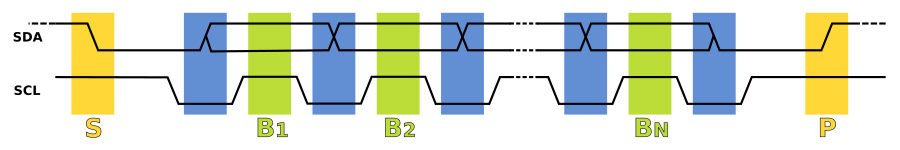
\includegraphics[width = 0.7\textwidth]{I2C_data_transfer.png}
            \caption{Ramka protokołu $I^2C$}
            \label{fig:i2c_data_frame}
            Źródło: \href{https://en.wikipedia.org/wiki/I%C2%B2C}{en.wikipedia.org/wiki/$I^2C$}
        \end{figure}

        W tym projekcie, powyższy standard wykorzystywany jest do komunikacji z trzema rodzajami urządzeń:
        \begin{table}[!ht]
            \centering
            \caption{Lista urządzeń podłączonych za pomocą $I^2C$}
            \begin{tabular}{|c|c|c|c|}\hline
                Nazwa      & Identyfikator & Adres $I^2C$ & Liczba\\
                urządzenia &   układu      &(hexadecymalnie)& modłów\\\hline
                Akcelerometr & \centerY{2}{MPU6050} & \centerY{2}{0x68} & \centerY{2}{1} \\
                i żyroskop   &&&\\\hline
                Magnetometr & QMC5883L & 0x0D & 1 \\\hline
                ToF & VL53L0 & 0x29 & 3 \\\hline
            \end{tabular}
        \end{table}

        W przypadku każdego z układów adres domyślny ustalany jest przez producenta.
        Konsekwencją podłączenia kilku takich samych komponentów do magistrali, może być konflikt transmisji - błędy podczas odczytywania danych.
        Dlatego producenci czasem umożliwiają zmianę adresu urządzenia docelowego.
        Wymaga to jednak zastosowania dodatkowych linii $xShut$, pozwalających na sekwencyjne uruchamianie czujników, w celu nadania im nowego identyfikatora.
        Procedura ta została wykorzystana do połączenia modułów ToF.

    \subsection{Protokół \texorpdfstring{$SPI$}{SPI}}
        Trzy- lub cztero- przewodowy protokół transmisji szeregowej, pozwalający na szybkie przesyłanie dużej ilości danych.
        Bardzo często używany do komunikacji z pamięcią zewnętrzną lub innym procesorem.
        Dokładny opis tej magistrali znajduje się w dokumencie \citetitle{SPI} \cite{SPI}.
        W tym projekcie pamięć zewnętrzną $W25Q32JV$ podłączono do mikrokontrolera za pomocą czteroprzewodowej odmiany tego standardu.
        % \cite{SPI_memory}.


    \subsection{Mostek H i sterowanie silnikami}
        Sterowanie silnikami odbywa się poprzez specjalne układy, tak zwane mostki H, które pozwalają na przepływ znacznego prądu.
        Kontrolę każdego silnika zapewniają trzy przewody: \textit{enable, in~1, in~2}, a odpowiednie stany opisuje tabela poniżej (tab \ref{tab:motor_control_state}).

        \begin{table}[!ht]
            \centering
            \caption{Schemat sterowania silnikiem}
            \label{tab:motor_control_state}
            \begin{tabular}{|c|c|c|c|}\hline
                \multicolumn{3}{|c|}{Stan przewodu:} & \centerY{2}{Stan silnika} \\\cline{1-3}
                \textit{Enable} & \textit{In 1} & \textit{In 2} & \\\hline
                L & x & x & Stop\\\hline
                H & L & L & Stop\\\hline
                H & L & H & Obroty w prawo\\\hline
                H & H & L & Obroty w lewo\\\hline
                H & H & H & Stop\\\hline
            \end{tabular}
        \end{table}
        gdzie:
        \begin{itemize}
            \item x -- stan dowolny,
            \item L -- stan niski - zero logiczne,
            \item H -- stan wysoki - jedynka logiczna.
        \end{itemize}

        Jak widać obsługa napędu jest prostym zadaniem, a dodatkowo podłączając sygnał PWM do wejścia \textit{enable}, można regulować prędkość silnika.
        Co więcej, do obu motorów dołączone są enkodery, połączone z procesorem za pomocą czterech przewodów.
        Raspberry Pi Pico nie posiada sprzętowych liczników, jednak kontroler PWM pozwala na maskowanie głównego zegara zewnętrznymi sygnałami, na przykład zboczem sygnału z enkodera.
        Dzięki temu można zliczać impulsy, wysyłane przez te układy.
        Na wykresie poniżej (rys. \ref{plot:speed_in_duty}) przedstawiono zależność prędkości silnika od wypełnienia sterowania na linii \textit{enable}.

        \begin{figure}[!ht]
            \centering
            \begin{tikzpicture}
                \begin{axis}[
                    width = 0.6\textwidth,
                    grid = both,
                    grid style = dashed,
                    xlabel = Wypełnienie PWM {[\%]},
                    ylabel = Prędkość {$[\frac{mm}{s}]$},
                    legend pos = south east,
                    ytick = {20, 40, ..., 200}
                ]
                    \addplot table [x = duty, y = speedL, col sep = comma]{Measure/speed.csv};
                    % \addplot table [x = duty, y = speedR, col sep = comma]{Measure/speed.csv};
                    % \legend{Lewy silnik, Prawy silnik}
                \end{axis}
            \end{tikzpicture}
            \caption{Wykres prędkości silników w zależności od wypełnienia sygnału PWM}
            \label{plot:speed_in_duty}
            Pomiar przeprowadzony przy napięciu zasilania mostka $6V$ \\
            i stałej częstotliwości $f_{PWM} = 25kHz$
        \end{figure}

    % \subsection{Serwomechanizm}
    %     Na schemacie z rysunku \ref{schema:block} literą $S$ oznaczono serwomechanizm, kontrolujący przednią oś pojazdu.
    %     Sterowanie modułem odbywa się za pomocą kontroli wypełnienia sygnału w zakresie od $150\mu s$ do $950\mu s$, pracującego na częstotliwości $f_{PWM} = 50Hz$.

    % \subsection{Czujniki cofania}
    %     Oba czujniki zostały podłączone bezpośrednio do mikroprocesora.
